
\let\negmedspace\undefined
\let\negthickspace\undefined
\documentclass[journal,12pt,twocolumn]{IEEEtran}
\usepackage{cite}
\usepackage{amsmath,amssymb,amsfonts,amsthm}
\usepackage{algorithmic}
\usepackage{graphicx}
\usepackage{textcomp}
\usepackage{xcolor}
\usepackage{txfonts}
\usepackage{listings}
\usepackage{enumitem}
\usepackage{mathtools}
\usepackage{gensymb}
\usepackage[breaklinks=true]{hyperref}
\usepackage{tkz-euclide} % loads  TikZ and tkz-base
\usepackage{listings}

\begin{document}


\vspace{3cm}

\title{
%	\logo{
AI5030-Probability Assignment 3
%	}
}
\author{ Samuktha V. (AI23MTECH02004)

	\thanks{*The author is with the Department
		of Dept. of AI, Indian Institute of Technology, Hyderabad
		502285 India e-mail:  ai23mtech02004@iith.ac.in. All content in this manual is released under GNU GPL.  Free and open source.}
}

% make the title area
\maketitle

\newpage


\textbf{Question 10.13.3.23 }
\newline
\textbf{Two dice are numbered 1, 2, 3, 4, 5, 6 and 1, 1, 2, 2, 3, 3, respectively. They are
thrown and the sum of the number yuils on them is noted. Find the probability of getting
each sum from 2 to 9 separately }
\newline
\newline
\textbf{\emph{Solution:} Solving using Convolution}
\newline
\newline
{ Let X be the discrete random variable corresponding to dice 1: \[ X \in \{1,2,3,4,5,6\} \]}

{ Let Y be the discrete random variable corresponding to dice 2: \[ Y \in \{1,1,2,2,3,3\} \]}
Let Z be the random variable that denotes the sum of the numbers when the above two dice are thrown.\[ Z \in \{2,3,4,5,6,7,8,9\} \] {
We need the sum \(z\), hence we take \( x \in X\) and sum over all possibilities of \(y\) where \(y=z-x \) so that sum is retained as \(z\).
The theoretical Probability Mass Function(PMF)  of Z can be generated using convolution operation as follows:
}
\begin{equation}\label{eq1}
   P_Z(z)=P(Z=z)= \sum_{x=1}^{6} P(X=x,Y=z-x)
\end{equation}
Since \(X\) and \(Y\) are independent, equation \ref{eq1} can be written as :
\[ P(Z=z)= \sum_{x=1}^{6} P(X=x) P(Y=z-x)\]
Hence,
\begin{equation}\label{eq2}
    P_Z(z)= \sum_{x=1}^{6} P_X(x)P_Y(z-x)
\end{equation}
The PMF of \(X\) and \(Y\) are plotted as shown in Figure \ref{pmf}:
\begin{figure}[!]
    \centering
    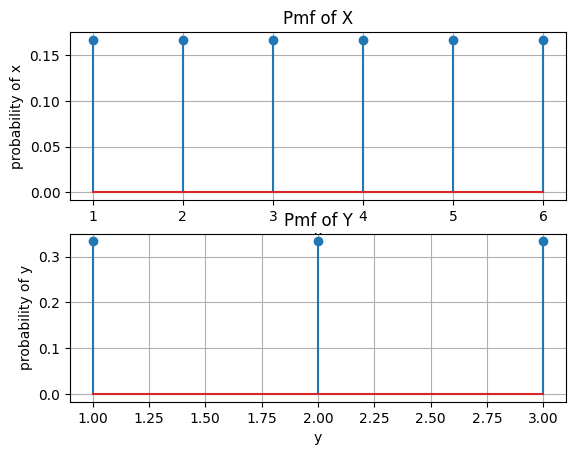
\includegraphics[scale=0.6]{pmf.png}
    \caption{PMFs of \(X\) and \(Y\)}
    \label{pmf}
\end{figure}\\
When \textbf{sum is 2}, we have 
\[P_Z(2)= \sum_{x=1}^{6} P(X=x)P(Y=2-x)=\frac{1}{18}\]
When \textbf{sum is 3}, we have 
\[P_Z(3)= \sum_{x=1}^{6} P(X=x)P(Y=3-x)=\frac{1}{9}\]

When \textbf{sum is 4}, we have 
\[P_Z(4)= \sum_{x=1}^{6} P(X=x)P(Y=4-x)=\frac{1}{6}\]

When \textbf{sum is 5}, we have 
\[P_Z(5)= \sum_{x=1}^{6} P(X=x)P(Y=5-x)=\frac{1}{6}\]

When \textbf{sum is 6}, we have 
\[P_Z(6)= \sum_{x=1}^{6} P(X=x)P(Y=6-x)=\frac{1}{6}\]

When \textbf{sum is 7}, we have 
\[P_Z(7)= \sum_{x=1}^{6} P(X=x)P(Y=7-x)=\frac{1}{6}\]

When \textbf{sum is 8}, we have 
\[P_Z(8)= \sum_{x=1}^{6} P(X=x)P(Y=8-x)=\frac{1}{9}\]

When \textbf{sum is 9}, we have 
\[P_Z(9)= \sum_{x=1}^{6} P(X=x)P(Y=9-x)=\frac{1}{18}\]
The PMF of X,Y and Z are shown in equation \ref{eq3},\ref{eq4} and \ref{eq5} respectively,
\begin{equation}\label{eq3}
     p_X(x) = \frac{1}{6} \hspace{1cm} for\hspace{0.5cm} 1\le x \le6
\end{equation}
\begin{equation}\label{eq4}
     p_Y(y) = \frac{1}{3} \hspace{1cm} for\hspace{0.5cm} 1\le<x\le3
\end{equation}
\begin{equation}\label{eq5}
    p_Z(z)=\begin{cases}
        \frac{1}{18}\hspace{1cm}for\hspace{0.5cm} z=2,9 \\
        \frac{1}{9} \hspace{1cm} for\hspace{0.5cm} z=3,8 \\
        \frac{1}{6} \hspace{1cm} for\hspace{0.5cm} 4\le z \le7 \\
    \end{cases}
\end{equation}
The pmf of Z is symmetrical and the distribution is plotted as shown in figure \ref{z} 
\begin{figure}[h]
    \centering
    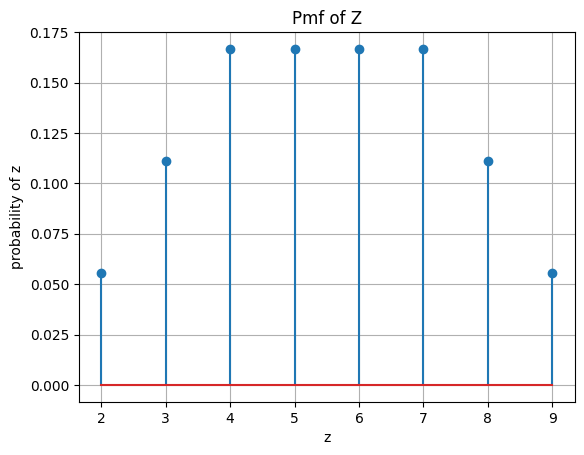
\includegraphics[scale=0.6]{pmf_z.png}
    \caption{PMF of \(Z\) }
    \label{z}
\end{figure}\\
\end{document}
